\documentclass[a4paper,12pt]{article}
\usepackage{graphicx}
\graphicspath{ {images/} }
\usepackage{float}
\usepackage[utf8]{inputenc}
\usepackage[english]{babel}
\usepackage[document]{ragged2e}
\usepackage{mathpazo}



\end{flushleft} 
\begin{document}\begin{flushleft}\newline \textbf{6.819 PSET 7}
\newline \textbf{11/10/2017}
\end{flushleft}
\newline \begin{center}\textbf{ISAAC KONTOMAH}
\end{center}
\begin{flushleft}
\newline \emph{Collaborators: Devin Morgan , Kamoya Ikhofua, Anthony Rolland , Benjamin Waar,Afika Nyati , Suman Nepal}
\end{flushleft}

\section{\emph{\textbf{ Photomerge}}}
\newline \textbf{a.} \emph{Plot of detected features and resulting correspondences}
\begin{document}
\newline Corresponding matches between Images

 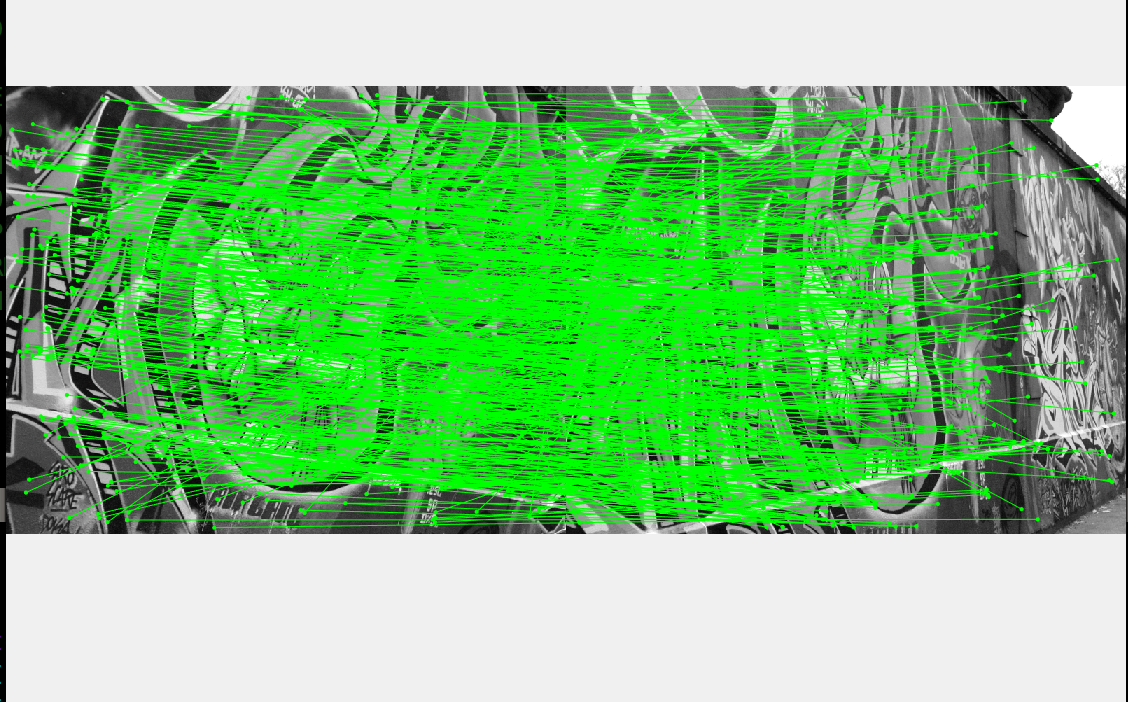
\includegraphics[height=5cm , width=8cm]{correspondence.jpg}

 \emph{Image showing corresponding matches between two images}
\newline \textbf{b.} \emph{Parameters of the TransformRANSAC algorithm}
\newline Number of Iterations : $10000$
\newline Threshold value : $0.6$
\newline $T$ matrix used \[
  \left[ {\begin{array}{ccc}
   -0.0030   &-0.0001   & 0.9173\\
   -0.0005   &-0.0027  &  0.3982 \\
   -0.0000  & -0.0000   &-0.0012 \\
  \end{array} } \right]
\]
\newline \textbf{d.} \emph{Panorama Image}
\begin{document}
\begin{figure}[H]
	\centering
	\begin{minipage}[b]{.5\linewidth}
		\centering
		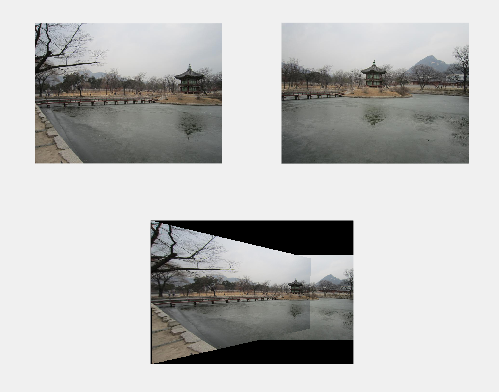
\includegraphics[width=8cm\linewidth, height=5cm]{seoul_pan.jpg}
		\caption{\emph{First Image panorama}}
	\end{minipage}
	\begin{minipage}[b]{.5\linewidth}
		\centering
		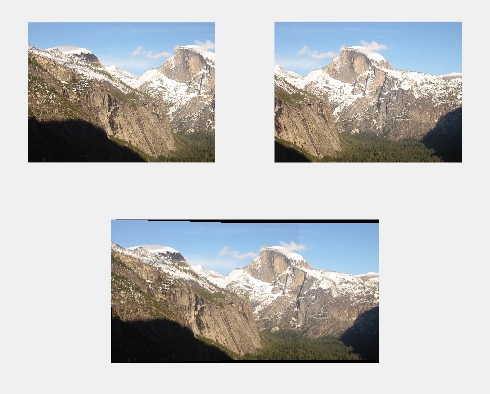
\includegraphics[width=8cm\linewidth, height=5cm]{mountains_pan.jpg}
		\caption{\emph{Second Image panorama}}
	\end{minipage}
\end{figure}

\end{document}